\documentclass[10pt,a4paper]{article}
\usepackage[utf8]{inputenc}
\usepackage[english]{babel}
\usepackage[T1]{fontenc}
\usepackage{amsmath}
\usepackage{amsfonts}
\usepackage{amssymb}
\usepackage{subcaption}
\usepackage{makeidx}
\usepackage{graphicx}
\usepackage{fourier}
\usepackage{listings}
\usepackage{color}
\usepackage{hyperref}
\usepackage[left=2cm,right=2cm,top=2cm,bottom=2cm]{geometry}
\author{Tommy Müller, Marcus Dittrich, Vincent Noculak}
\title{Zeeman-Effekt}

\lstset{language=C++,
	keywordstyle=\bfseries\color{blue},
	commentstyle=\itshape\color{red},
	stringstyle=\color{green},
	identifierstyle=\bfseries,
	frame=single}
\begin{document}

\maketitle
\newpage
\tableofcontents
\newpage

\section{Theorie}

\section{Durchführung}

In dem Versuch sollte der normale Zeeman-Effekt beobachtet werden. Abbildung \ref{aufbau} zeigt den Aufbau des Versuchs. Mit Hilfe einer Quecksilber-Spektrallampe, die sich für Teile der Messung in einem Magnetfeld befindet, wird Licht erzeugt. Dieses wird durch eine Sammellinse gebündelt und durch einen Monochromator geleitet, mit dessen Hilfe bestimmte Spektrallinien des Lichts gezielt durchgelassen werden können. Das vom Monochromator durchgelassene Licht läuft dann durch eine Linse, gefolgt von einem Fabry-Perot-Interferometer. Durch eine Kamera kann das Licht nach dem Fabry-Perot-Interferometer am Computer untersucht werden. 

Der Versuch begann damit, das Spektrum der Quecksilber-Spektrallampe bei noch ausgeschaltetem Magnetfeld mit Hilfe des Monochromators zu beobachten. Daraufhin wurde unter Beobachtung der grünen Spektrallinie der Strahlengang auf optimale Schärfe justiert. Hierzu wurden die vom Fabry-Perot-Interferometer erzeugten Ringe betrachtet und darauf hin aufgenommen.

Jetzt wurde das Magnetfeld angeschaltet, um den normalen Zeeman-Effekt zu untersuchen. Ausgehend von der grünen Spektrallinie, wurde die Polarisation der Zeeman-Komponenten und die Aufspaltung der Spektrallinie abhängig von der Stärke des Magnetfelds beobachtet.

\begin{figure}[h]
	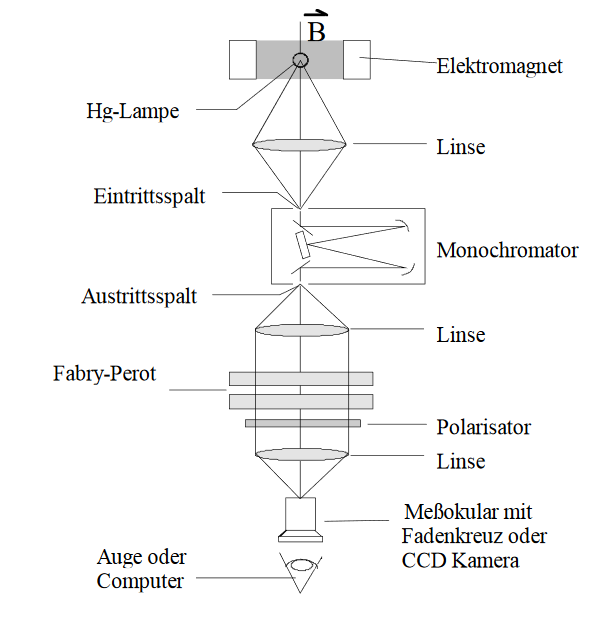
\includegraphics[scale = 1]{Zeeman_aufbau.png}
	\centering
	\caption{Versuchsaufbau, Quelle: Versuchsanleitung vom Zeeman-Effekt-Versuch des Fortgeschrittenenpraktikums}
	\label{aufbau}
\end{figure}

\section{Versuchsauswertung}

Mit dem Monochromator hatten wir zum Beginn des Versuchs das Feinstrukturspektrum der Quecksilber-Spektrallampe von $400nm$
bis $900nm$ beobachtet. An dem Monochromator konnte per Rad die durchgelassene Wellenlänge eingestellt werden. Eine Angabe zu der Durchlassgenauigkeit des Monochromators konnten wir nicht finden. In Tabelle \ref{spektrum} können die von uns beobachteten Spektralfarben gesehen werden. Wir waren in der Lage, die meisten Spektralfarben mit einer Abweichung von höchstens 4 Nanometern wahrzunehmen. Die cyanfarbige und rote Spektrallinie konnten wir nicht beobachten. Es fällt auf, dass die von uns beobachteten Spektrallinien immer ein paar Nanometer über den tatsächlichen Literaturwerten gemessen worden sind. Dies könnten an einem systematischen Fehler am Monochromator liegen.

Die bei $577nm$ und $579nm$ liegenden orangenen Spektrallinien der Spektrallampe konnten wir nur als einzelne Linie bei $580nm$ wahrnehmen.

\begin{table}[h!]
	\centering
\begin{tabular}{|l|r|c|lrp{16cm}}\hline
	Farbe & Literaturwerte in nm & Beobachtete Wellenlängen in nm\\\hline
	Violett & 405 & 409\\
	Blau & 436 & 439\\
	Cyan & 492 & -\\
	Grün & 546 & 548\\
	Orange & 577 & 580\\
	Orange & 579 & 580\\
	Rot & 615 & -\\\hline
\end{tabular}
	\caption{Beobachtete Spektrallinien der Quecksilber-Spektrallampe}
	\label{spektrum}
\end{table}


\subsection{Bestimmung der Frequenzaufspaltung}

%Die Nummer der Formel muss noch hinzugefügt werden
Die Frequenzaufspaltung durch das Magnetfeld kann mit Hilfe von Formel ref Bestimmt werden. Der dazugehörige Fehler lässt sich mit den Gesetzen der Fehlerfortpflanzung als folgenden bestimmen:

\begin{equation}
\Delta\Delta\nu = \frac{c}{\lambda} \sqrt{(\frac{r_1}{f^2} \cdot\Delta r_1)^2 + (\frac{-r_2}{f^2}\cdot \Delta r_2)^2 + (\frac{r_1^2 - r_2^2}{f^3} \cdot \Delta f)^2)}
\label{fehler123}
\end{equation}
 Wir haben die Aufspaltung des grünen Lichts der Spektrallampe gemessen. Aus Tabelle \ref{spektrum} kann abgelesen werden, dass das grüne Licht eine Wellenlänge von $546 nm$ hat. Die Brennweite der verwendeten Linse, die wir zur Berechnung der Frequenzaufspaltung benötigen, haben wir schon berechnet.
%, sie beträgt...
Die Zeeman-Aufspaltung $\Delta\nu$ einer Spektrallinie ist nach oben die gleiche, wie nach unten. Deshalb können wir zur Berechnung der Aufspaltung den Ring im Interferometer mit kleinerem und höherem Radius nehmen(Von den 3 Ringen gleicher Ordnung) und zum Schluss die damit berechnete Frequenzaufspaltung durch 2 teilen. Den jeweils dritten Ring mit durch den Zeeman-Effekt unverändertem Radius müssen wir nicht beachten. Wir benutzen bei den verschiedenen Magnetfeldstärken jeweils die Radien der Ringe der ersten Ordnung. 
Mithilfe der vorgegebenen Eichkurve aus der Versuchsanleitung können die zu unseren gemessenen Strömen zugehörige Magnetfelder bestimmt werden. (Tabelle \ref{gemessene_frequenzaufspaltungen}).

Der Zusammenhang zwischen der Frequenzaufspaltung und der Wellenzahlaufspaltung durch den Zeeman-Effekt ist gegeben durch $\Delta k = \frac{2 \cdot \pi}{c} \cdot \Delta\nu$.

Die berechnete Frequenzaufspaltung in GHz und $cm^{-1}$ können in Tabelle \ref{gemessene_frequenzaufspaltungen} gesehen werden.
%Ergebnis kommentieren

Da wir nun Messergebnisse der Frequenzaufspaltungen für verschieden starke Magnetfelder haben, können wir diese gegenüber in einem Diagramm Auftragen. Die Ausgleichsgeraden, sowie die Grenzgeraden wurden mithilfe linearer Regression berechnet. Hier hat die obere Grenzgrade die Steigung $b + \Delta b$ und schneidet die y-Achse bei $a + \Delta a$ und die untere Grenzgerade hat die Steigung $b - \Delta b$ und schneidet die y-Achse bei $a - \Delta a$. Die berechneten Werte für $b$, $\Delta b$, $a$ und $\Delta a$ können in Tabelle \ref{diagramm_werte} gesehen werden.
 Wir betrachten ein Diagramm von $\Delta\nu$ gegen $B$ in \ref{diagramm_aufspaltung} und eins von $\Delta k$ gegen $B$. Weil sich $\nu$ und $k$ nur um einen Vorfaktor unterscheiden, reicht es, wenn wir nur \ref{diagramm_aufspaltung} betrachten.
Weil die Frequenzaufspaltung des Zeeman-Effekts proportional zu $B$ ist, sollte bei einer perfekten Messung die Gerade durch den Koordinatenursprung gehen.

\begin{table}[h!]
	\centering
	\begin{tabular}{|l|r|c|lrp{16cm}}\hline
		Strom in A & Dazugehöriges Magnetfeld in T & $\Delta \nu$ in GHz & $\Delta k$ in $cm^{-1}$ \\\hline
		10 & 0,48 & 3,8 $\pm$ 6,7& 0,8 $\pm$ 1,4\\
		12 & 0,57 & 5,8  $\pm$ 6,9& 1,2 $\pm$ 1,4\\
		14 & 0,66 & 7,3 $\pm$ 7,1& 1,5 $\pm$ 1,5\\
		16 & 0,75 & 8,7 $\pm$ 7,3& 1,8 $\pm$ 1,5\\
		18 & 0,82 & 9,5 $\pm$ 7,4& 1,9 $\pm$ 1,6\\
		20 & 0,89 & 10,1 $\pm$ 7,5& 2,1 $\pm$ 1,6\\\hline
	\end{tabular}
	\caption{Durch die Eichkurve bestimmte Magnetfelder für bestimmt Stromstärken}
	\label{gemessene_frequenzaufspaltungen}
\end{table}



\begin{figure}[h]
	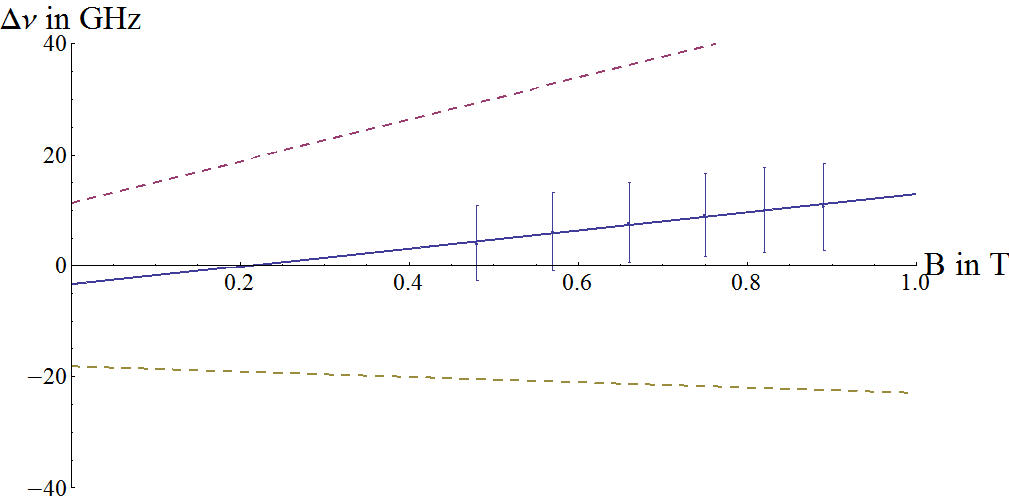
\includegraphics[scale = 0.5]{frequenzaufspaltung.png}
	\centering
	\caption{Durch den Zeeman-Effekt hervorgerufene Frequenzaufspaltung, abhängig vom Magnetfeld}
	\label{diagramm_aufspaltung}
\end{figure}
\begin{figure}[h]
	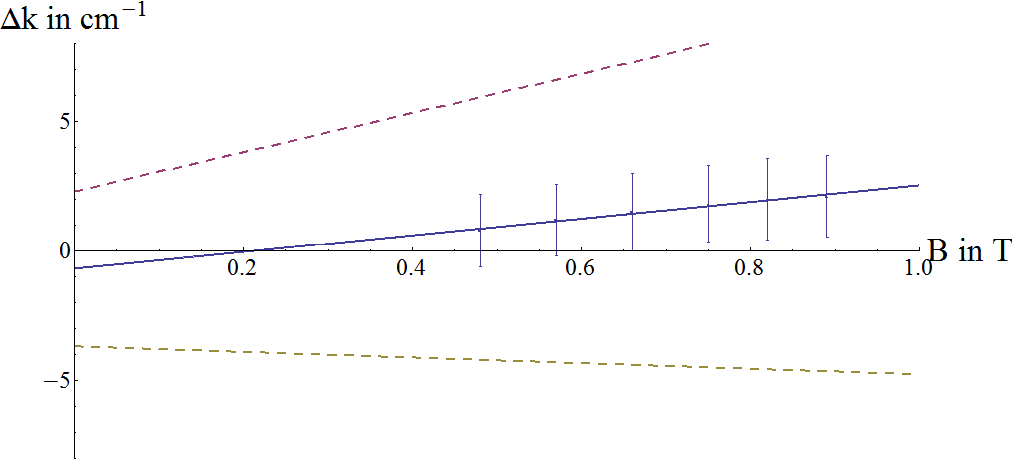
\includegraphics[scale = 0.5]{wellenzahlaufspaltung.png}
	\centering
	\caption{Durch den Zeeman-Effekt hervorgerufene Wellenzahlaufspaltung, abhängig vom Magnetfeld}
	\label{diagramm_aufspaltung_wellenzahl}
\end{figure}


\begin{table}[h!]
	\centering
	\begin{tabular}{|l|r|c|lrp{16cm}}\hline
		Steigung in $\frac{GHz}{T}$ & a in $GHz$\\\hline
		$15 \pm 20$ & $-3 \pm 14$\\\hline
	\end{tabular}
	\caption{Steigung b und Achsenabschnitt a  des Diagramms $\Delta\nu$ gegen $B$}
	\label{diagramm_werte}
\end{table}



Die durch den Zeeman-Effekt hervorgerufene Energiedifferenz zwischen zwei Atomzuständen mit gleicher Haupt- und Nebenquantenzahl ist gegeben durch

\begin{align}
	E_{mj+1}- E_{mj} = \Delta E_{Zeeman} = g_j \mu_B B \\
	\Rightarrow h \Delta \nu =  g_j \mu_B B \\
	\Rightarrow \Delta \nu = \frac{g_j \mu_B}{h} B
	\label{steigungnu}
\end{align}

\subsection{Bestimmung von $g_j$}

In \ref{steigungnu} kann sehen, dass wenn die Frequenzaufspaltung des Zeeman-Effekts gegen die Stärke des Magnetfelds aufgetragen wird, durch die Steigung der sich dadurch ergebenen Geraden der Lande-Faktor $g_j$ bestimmt werden kann. Ist die Steigung $b$ der Geraden, so ist der Lande-Faktor gegeben durch

\begin{equation}
g_j = \frac{b \cdot h}{\mu_B}
\end{equation}

Somit erhalten wir für $g_j$ mit unseren Ergebnissen aus Tabelle \ref{diagramm_werte} einen Wert von $1,1 \pm 1,4$. Theoretisch ist $g_j$ gegeben durch

\begin{equation}
 g_j = 1 + \frac{j(j+1) + s(s+1) - l(l+1)}{2 j(j+1)}
 \label{lande2}
\end{equation}

Die Emission des grünen Lichts($546 nm$) einer Quecksilberdampflampe entspricht dem Übergang vom Zustand $^3S_1$ nach $^3P_2$ eines Quecksilberatoms. Der mit \ref{lande2} berechnete Wert für $g_j$ des ersteren Zustands ist $g_j = 2$ und für den letzteren Zustand $g_j =1,5$ je nachdem, welchen Wert j annimmt. Unser Berechneter Wert muss deshalb im Bereich $1,5-2$ sein. Der theoretische Wert von $g_j$ stimmt damit mit unseren berechneten überein.



\section{Diskussion}

Der von uns beobachtete Zeeman-Effekt stimmte mit der Theorie überein. Die Spektrallinien der Quecksilberdampflampe spalteten sich nach Anschalten den Magnetfelds in jeweils drei Linien auf, wovon zwei zirkular und eins linear polarisiert waren. Mit dem Fabry-Perot-Interferometer wurde anhand der Bestimmung von den Radien der Inteferenzmaxima die Frequenzaufspaltung des Zeeman-Effekts gemessen. Nach einer grafischen Darstellung der Frequenzaufspaltung gegen die Magnetfeldstärke, konnte man sehen, dass sich unter Berücksichtigung der Messfehler, eine Ursprungsgerade ausbildete, wie von der Theorie vorhergesagt(\ref{steigungnu}). Aus der Ursprungsgerade konnte aus der Steigung der Gerade $g_j$ bestimmt werden, welches identisch mit dem theoretischen Wert $g_j$'s ist. Weil wir so große Fehler haben, die teilweise größer, als die gemessenen Werte an sich sind(siehe $g_j$), sind unsere Messwerte sehr wenig aussagekräftig. Die Größe, der von uns angegebenen Messfehler sind gut in den Diagrammen veranschaulicht. In den Diagrammen, sieht man auch anhand der Linearität der Messwerte, dass unsere angegebenen Messfehler wahrscheinlich größer, als die tatsächlichen Messfehler sind.


Zusammenfassend lässt sich sagen, dass unsere Messungen zwar gut geeignet sind, die theoretischen Vorhersagen des Zeeman-Effekts zu verifizieren, sich konkrete Werte wegen den großen Messfehlern, nur sehr ungenau bestimmen lassen.


\end{document}